\documentclass[12pt]{article}%
\usepackage{graphicx}
\usepackage{ragged2e}
\usepackage{indentfirst}
\usepackage{float}
%\usepackage{setspace}
%\usepackage{subfigure}
\usepackage{amsmath}
\usepackage{amsfonts}
%\usepackage{amssymb}
%\usepackage{amsbsy}
%\usepackage{times}
\usepackage[colorlinks=true,citecolor=black,linkcolor=black]{hyperref}
%\usepackage{multirow}
%\usepackage{booktabs}
\usepackage[english]{babel}
\usepackage[utf8]{inputenc}
\usepackage{fancyhdr}
\usepackage{listings}
\usepackage{color}
%
\definecolor{codegreen}{rgb}{0,0.6,0}
\definecolor{codegray}{rgb}{0.5,0.5,0.5}
\definecolor{codepurple}{rgb}{0.58,0,0.82}
\definecolor{backcolour}{rgb}{0.95,0.95,0.92}
\lstdefinestyle{mystyle}{
    backgroundcolor=\color{backcolour},   
    commentstyle=\color{codegreen},
    keywordstyle=\color{magenta},
    numberstyle=\tiny\color{codegray},
    stringstyle=\color{codepurple},
    basicstyle=\footnotesize,
    breakatwhitespace=false,         
    breaklines=true,                 
    captionpos=b,                    
    keepspaces=true,                 
    numbers=left,                    
    numbersep=5pt,                  
    showspaces=false,                
    showstringspaces=false,
    showtabs=false,                  
    tabsize=2
}
\lstset{style=mystyle}
%
\pagestyle{fancy}
\fancyhf{}
\rhead{Spring 2017}
\lhead{CALVIN \& PyVIN Shortcourse}
\cfoot{\thepage}
\rfoot{\textit{\small updated on \today}}
% 
\begin{document}
%
\title{\textbf{CALVIN \& PyVIN} Shortcourse}
%
\date{April 1, 2017}
\author{
Mustafa S. Dogan
%
\thanks{
Graduate Student,
Dept.\ of Civil and Env. Eng.,
Univ.\ of California, Davis, 
1 Shields Avenue,
Davis, CA  95616. E-mail: msdogan@ucdavis.edu.},
}
%
\maketitle
%
\tableofcontents
%
\pagebreak
%
\begin{center}
	{\bf \Huge{Agenda and Topics \\}}
\end{center}
%
\hrule
\begin{table}[h]
    \centering
    %\caption{\huge agenda & topics}
    \label{agenda}
    \begin{tabular}{lll}
         15 min &\textendash & Introduction and set-up \\
         1 hr &\textendash & CALVIN theory and model introduction \\
         \bf{15 min} &\textendash & \bf{Break} \\
         15-20 min &\textendash & HOBBES database \\
         15 min &\textendash & Data flow overview \\
         \bf{1 hr} &\textendash & \bf{Break} \\
         20-25 min &\textendash & PyVIN updates and model architecture\\
         15 min &\textendash & A PyVIN example \\
         \bf{15 min} &\textendash & \bf{Break} \\
         15-20 min &\textendash & Required software and installation \\
         20 min &\textendash & Your first PyVIN run \\
         20-25 min &\textendash & Postprocessing results
    \end{tabular}
\end{table}
\hrule
%
\pagebreak
\section{Prerequisites}
Please bring your \textbf{laptop} with below software dependencies installed if you want a hands-on PyVIN experience. Install following software in advance since some of them, such as Anaconda, takes long time to download and install. If you have any question, e-mail msdogan@ucdavis.edu
%
\begin{itemize}
	\item {\bf Python v3 with Anaconda} \\ Link: https://www.continuum.io/downloads
	\begin{figure}[H]
		\centering
    		\includegraphics[width=0.5\linewidth]{anaconda.pdf}
   		\caption{Anaconda package for Windows and Mac OS}
    		\label{fig:anaconda}
	\end{figure}
	Note: Download Python v3+ (not v2.7) because Pyomo command line installation works only with Python v3+
	\item {\bf GitHub} \\ Link: https://desktop.github.com
	\begin{figure}[H]
		\centering
    		\includegraphics[width=0.45\linewidth]{github.pdf}
   		\caption{GitHub installation for Windows and Mac OS}
    		\label{fig:github}
	\end{figure}
	\item {\bf Pyomo} \\ Command: {\tt \small conda install -c cachemeorg pyomo pyomo.extras glpk}
\end{itemize}
%
Note: if you don't know how to use command line, please refer to description below and then type the command.
\subsection{Command line}
%
This shortcourse is not intended to explain command line use. It assumes some but not extensive command line knowledge. If you like to learn basics of command line, here is a nice crash course:
%
\par https://learnpythonthehardway.org/book/appendixa.html
%
\begin{figure}[H]
    \centering
    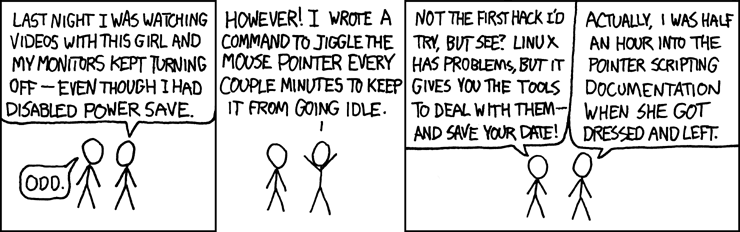
\includegraphics[width=1\linewidth]{command_line_fu.png}
    \caption{A command line comic from xkcd, source: https://xkcd.com/196/}
    \label{fig:command_line}
\end{figure}
%
\subsubsection{Windows}
%
After installing GitHub, double click on "Git Shell" and then type the command above to install Pyomo and GLPK solver.
%
\begin{figure}[H]
		\centering
    		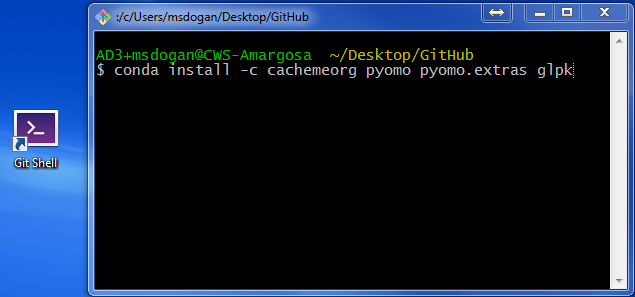
\includegraphics[width=0.6\linewidth]{Capture.png}
   		\caption{Command line (Git Shell) for Windows}
    		\label{fig:gitshell}
\end{figure}
%
\subsubsection{Mac OS}
%
Search "terminal" in Spotlight Search and then double click. Type the command above to install Pyomo and GLPK solver.
\begin{figure}[H]
		\centering
    		\includegraphics[width=0.6\linewidth]{terminal.pdf}
   		\caption{Command line (terminal) for Mac OS}
    		\label{fig:terminal}
\end{figure}
%
\pagebreak
%
\section{Introduction and background}
%
Developed in early 2000s, {\bf CAL}ifornia {\bf V}alue {\bf IN}tegrated model (CALVIN) combines ideas from economics and engineering optimization with advances in software and data to suggest more integrated management of water supplies regionally and throughout California. CALVIN is an hydro-economic optimization model for California's advanced water infrastructure that integrates the operation of water facilities, resources, and demands, and it aims to optimize surface and groundwater deliveries to agricultural and urban water users. It allocates water to maximize statewide agricultural and urban economic value, considering physical and policy constraints. It replicates water market operations transferring water from users with lower willingness-to-pay (WTP) to users with higher WTP. CALVIN uses historical hydrology and 2050 water demand projections for its operations. Figure \ref{fig:coverage} regions and coverage of the model. \\
\par CALVIN forces quantitative understanding of integrated water and economic system. Motivation for the CALVIN effort include:
\begin{itemize}
	\item making better sense of integrated system and operations
	\item seeking ways to improve system management
	\item quantifying user willingness to pay for additional water
	\item finding insights into changes in physical capacities and policies
\end{itemize}
%
\par With the recent updates, CALVIN is evolved to open-source PyVIN model, optimizing water resources in a short amount of time with state-of-the-art solvers and modeling platform. PyVIN has the same input data and objective as CALVIN but it is modeled on Pyomo, a Python-based high level algebraic modeling language. PyVIN also uses HOBBES database, which allows better documentation, collaboration and communication between models as well as modelers.
%
\begin{figure}[H]
    \centering
    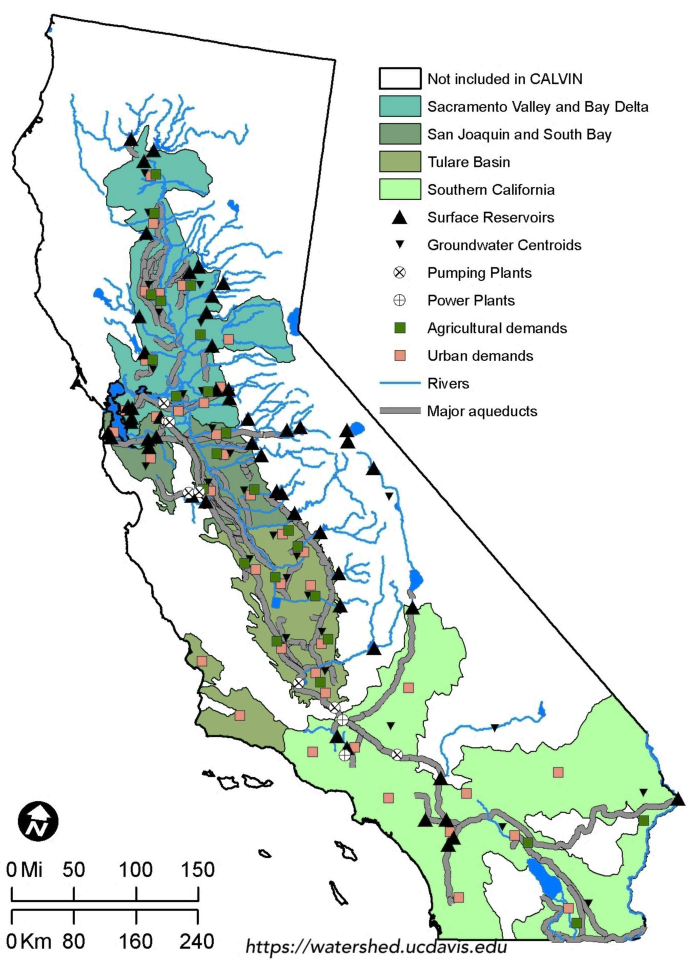
\includegraphics[width=0.9\linewidth]{coverage.pdf}
    \caption{California's water infrastructure and CALVIN's coverage}
    \label{fig:coverage}
\end{figure}
%
\section{HOBBES database}
%
HOBBES serves as a cross-platform for data storage, display and documentation. It is a framework for database that aims to better organize data and makes model integration and communication easier by using common format and metadata. Classical approach in modeling is that first model is built and then required data are collected. But HOBBES reverses this order; it serves as a data hub and models are built on top of this database. HOBBES uses GitHub to keep track of changes and documentation. It also has a animation tool to display data.
%
\begin{figure}[H]
    \centering
    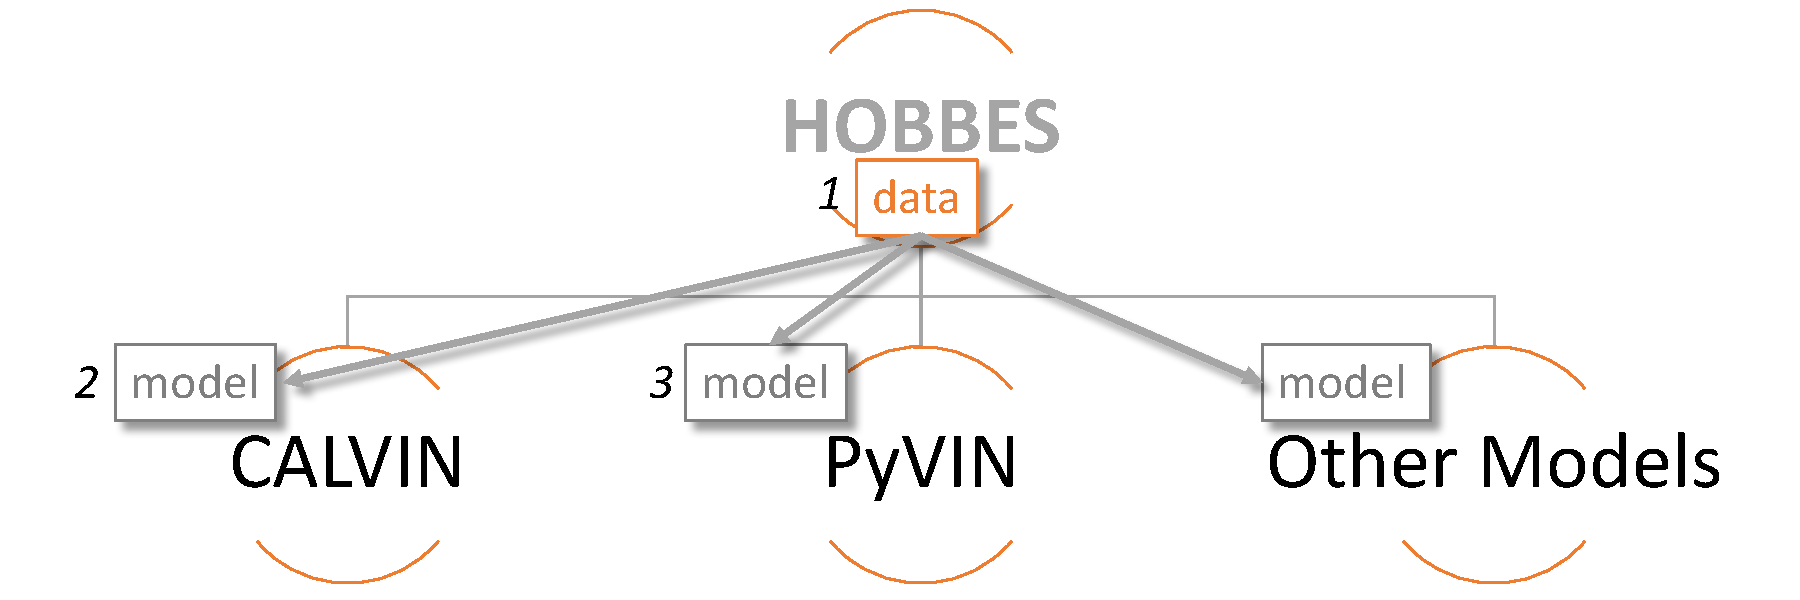
\includegraphics[width=0.6\linewidth]{hobbes.pdf}
    \caption{HOBBES database and model integration}
    \label{fig:hobbes}
\end{figure}
%
\subsection{Data flow overview}
%
\begin{figure}[H]
    \centering
    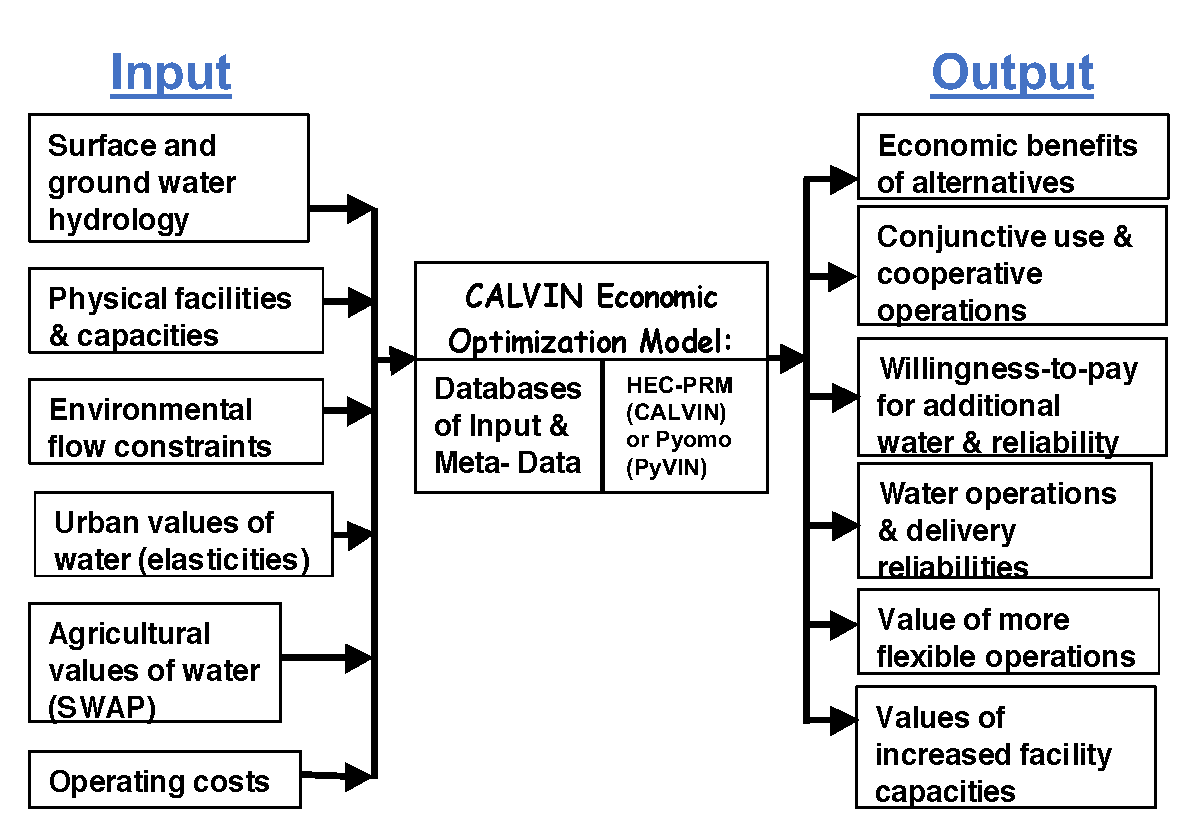
\includegraphics[width=0.7\linewidth]{dataflow.pdf}
    \caption{CALVIN (and PyVIN) data overflow with input (left column) and output (right column)}
    \label{fig:dataflow}
\end{figure}
%
\section{Updated version: PyVIN}
%
PyVIN combines CALVIN's knowledge and extensive water infrastructure and hydrology data with a high level algebraic modeling language, Pyomo, and state-of-the-art solvers, such as CPLEX, Gurobi, CBC, and GLPK. Pyomo is an open-source Python based large-scale modeling environment. Its model representation is similar to GAMS and AMPL and it solves the problem with user defined solvers. So, PyVIN is not solver specific and users can choose and install any solver as long as it is compatible with Pyomo.
%
\begin{figure}[H]
    \centering
    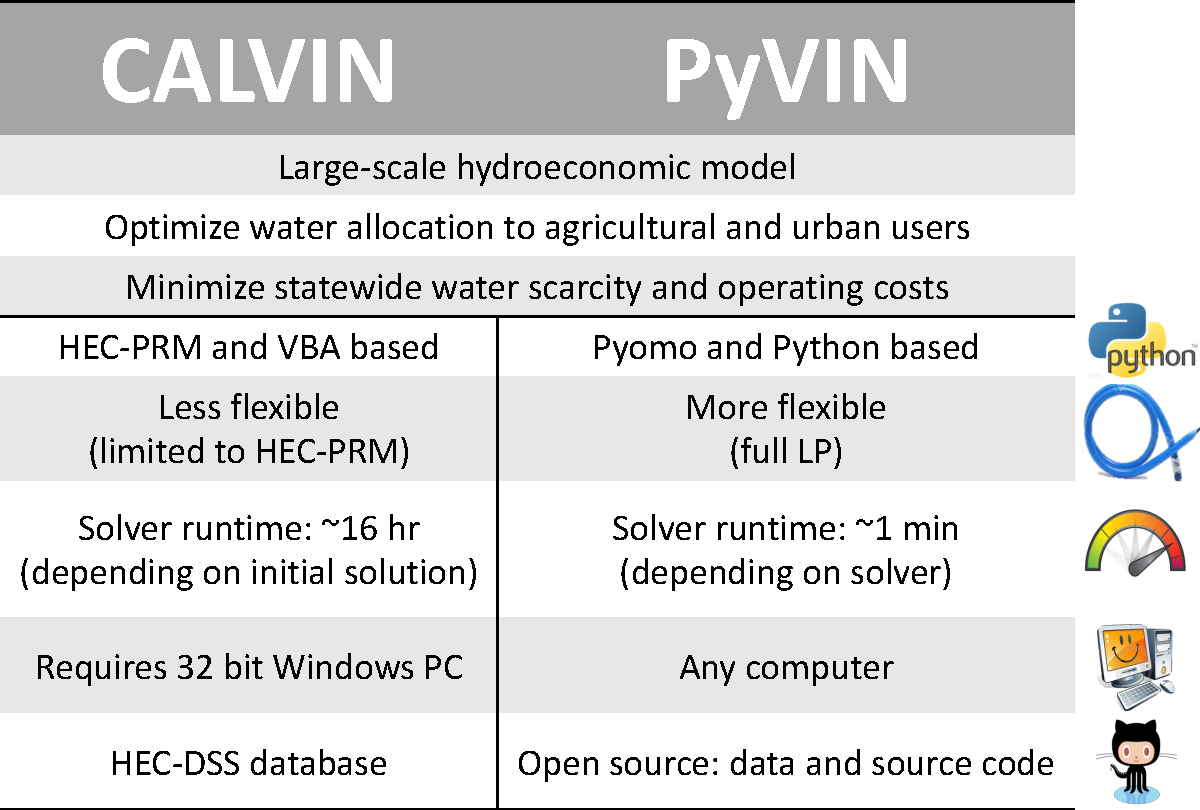
\includegraphics[width=0.6\linewidth]{comparison.pdf}
    \caption{CALVIN (and PyVIN) data overflow with input (left column) and output (right column)}
    \label{fig:comparison}
\end{figure}
%
\subsection{Model architecture}
%
Modeled in different environments, both CALVIN and PyVIN solve the same objective function, subject to physical and environmental constraints. The objective is to minimize statewide water scarcity and operating costs (Equation \ref{eq:obj}). There are three constraints: upper bound (Equation \ref{eq:upper}), lower bound (Equation \ref{eq:lower}), and mass balance (Equation \ref{eq:mass}).
%
\begin{equation} \label{eq:obj}
max (z) = \sum_{i}\sum_{j}\sum_{k} c_{ijk}X_{ijk}
\end{equation}
%
\begin{equation} \label{eq:upper}
X_{ijk} \leq u_{ijk}
\end{equation}
%
\begin{equation} \label{eq:lower}
X_{ijk} \geq l_{ijk}
\end{equation}
%
\begin{equation} \label{eq:mass}
\sum_{j}\sum_{i} X_{ijk} = \sum_{i}\sum_{j} a_{ijk}X_{ijk} + b_j
\end{equation}
%
where $c$ represents unit cost, $X$ is flow, $u$ is upper bound, $l$ is lower bound, $a$ is amplitude to represent losses, and $b$ is a local inflow to node $j$.
\par PyVIN is modeled as an abstract model in Pyomo, separating model structure from data. PyVIN can solve any data size and data do not have to be water resources. As long as it is a network flow problem, such as transportation or transmission, PyVIN can solve it. Also, since it is open-source and has full linear programming features, it has more flexible model representation. Any other constraints can easily be added in addition to three constraint mentioned before. The Pyomo structure code with parameters and equations is shown below.
%
\begin{lstlisting}[language=Python]
from __future__ import division 
from pyomo.environ import *
import itertools

model = AbstractModel()

# Nodes in the network
model.N = Set()

# Network arcs
model.k = Set()

model.A = Set(within=model.N*model.N*model.k)

# Source node
model.source = Param(within=model.N)
# Sink node
model.sink = Param(within=model.N)

# Flow capacity limits
model.u = Param(model.A)
# Flow lower bound
model.l = Param(model.A)
# Link amplitude (gain/loss)
model.a = Param(model.A)
# Link cost
model.c = Param(model.A)

# The flow over each arc
model.X = Var(model.A, within=Reals)

# Minimize total cost
def total_rule(model):
    return sum(model.c[i,j,k]*model.X[i,j,k] for (i,j,k) in model.A)
model.total = Objective(rule=total_rule, sense=minimize)

# Enforce an upper bound limit on the flow across each arc
def limit_rule_upper(model, i, j, k):
    return model.X[i,j,k] <= model.u[i,j,k]
model.limit_upper = Constraint(model.A, rule=limit_rule_upper)

# Enforce a lower bound limit on the flow across each arc
def limit_rule_lower(model, i, j, k):
    return model.X[i,j,k] >= model.l[i,j,k]
model.limit_lower = Constraint(model.A, rule=limit_rule_lower)

# Enforce flow through each node (mass balance)
def flow_rule(model, node):
  if node in [value(model.source), value(model.sink)]:
      return Constraint.Skip
  outflow  = sum(model.X[i,j,k]/model.a[i,j,k] for i,j,k in model.A)
  inflow = sum(model.X[i,j,k] for i,j,k in model.A)
  return inflow == outflow
model.flow = Constraint(model.N, rule=flow_rule)
\end{lstlisting}
%
\par The data file {\tt data.dat} includes list of nodes, and list of links with properties. All links have cost $c$, amplitude $a$, lower bound $l$, and upper bound $u$. Below is an example data file.
%
\begin{lstlisting}
set N :=
INITIAL	SR_SHA.1983-10-31	SR_SHA.1983-11-30		FINAL	
INFLOW.1983-10-31	INFLOW.1983-11-30	...;

set k := 0 1 2 3 4 5 6 7 8 9 10 11 12 13 14 15;

param source := SOURCE;
param sink := SINK;

param: A: c a l u :=
SOURCE	INITIAL	0	0	1	0	10000000
INITIAL	SR_SHA.1983-10-31	0	0	1	3686.84	3686.84
SR_SHA.1983-10-31	SR_SHA.1983-11-30	0	-7.003	0.997	630.4	630.4
SR_SHA.1983-10-31	SR_SHA.1983-11-30	1	-2.974	0.997	737.4	737.4
SR_SHA.1983-10-31	SR_SHA.1983-11-30	2	-1.466	0.997	632.2	2032.2
SR_SHA.1983-11-30	SR_SHA.1983-12-31	0	-6.972	0.999	609.4	609.4
SR_SHA.1983-11-30	SR_SHA.1983-12-31	1	-3.056	0.999	700.8	700.8
SR_SHA.1983-11-30	SR_SHA.1983-12-31	2	-1.479	0.999	689.7	1941.7
FINAL	SINK	0	0	1	0	10000000
SR_SHA.1984-09-30	FINAL	0	0	1	2923.297	2923.297
SOURCE	INFLOW.1983-10-31	0	0	1	0	10000000
INFLOW.1983-10-31	SR_SHA.1983-10-31	0	0	1	301.765	301.765
SOURCE	INFLOW.1983-11-30	0	0	1	0	10000000
\end{lstlisting}
%
\section{Your first model run}
%
\subsection{Postprocessing results}
%
\section{References and useful links}
\end{document}